\chapter{Pointer and Effect Analysis}
\label{chap:pointer}
The problem of analyzing pointers is closely related to the field of effects
analysis. Indeed, establishing the relations between pointers require
understanding how and to what values fields are written to. Because of this
strong inter-dependence, it is often profitable to perform both simultaneously.

Our analysis builds summaries of methods, both in terms of effects and shape of
the heap. Those summaries are stored in graphs. In order that compute the
resulting graphs for each method, we perform a flow-sensitive
abstract-interpretation based analysis. A graph is thus associated to each
program point. The next section describes how those graphs are generated and
what their semantics are. This representation is similar in many aspects to
the graph representation used by Alexandru Salcianu in his Thesis. We can %FIXME
however point out two important differences: his work is primarily focused on
escape analysis, our isn't and thus we do not keep escape-specific information
in our abstract representation. We also introduced multiple kinds of global
nodes, that were not present in his work since it would be redundant for escape
analysis. Although the representations are similar, the semantics of our graphs
as well as the procedures to build them differ.

\section{Graph Semantics}
Our representation is based on labelled directed graphs augmented with some
metadata. They are defined by:
\begin{eqnarray*}
    G           := &\langle& N \subseteq Nodes, \\
                   && E \subseteq Edges, \\
                   && locVar \subseteq Variables \times \mathcal{P}(N), \\
                   && Ret \subseteq N ~ \rangle \\
    Edges       := && IEdges \cup OEdges  \\
    IEdges      := && \langle N, f, N \rangle \in Nodes \times Fields \times Nodes ~\textsf{ Inside Edges } \\
    OEdges      := && \langle N, f, N \rangle \in Nodes \times Fields \times Nodes ~\textsf{ Outside Edges } \\
    Variables   := && \textsf{All local variables and arguments} \\
    Fields      := && \textsf{Field names} \\
    Nodes       := && \{ GBNode, NNode \} \cup INodes \cup LNodes \\
                   && \cup PNodes \cup OBNodes \cup LitNodes \\
    INodes      := && \langle T \rangle \in TypeInfo ~ \textsf{(Allocation node)} \\
    LNodes      := && \langle from, via, T \rangle \in Nodes \times Fields \times TypeInfo ~ \textsf{(Load node)} \\
    PNodes      := && \langle i, T \rangle  \in \mathbb{R} \times TypeInfo ~ \textsf{(Param node)} \\
    OBNodes     := && \langle T \rangle \in TypeInfo ~ \textsf{(Object Node)} \\
    LitNodes    := && \langle T \rangle \in TypeInfo ~ \textsf{(Literal values of primitive types)} \\
    NNode       := && ~ \textsf{(Null node)} \\
    GBNode      := && ~ \textsf{(Global node)} \\
\end{eqnarray*}

Nodes generally represent sets of objects (including literals of primitive
types), while edges represent may/must-point-to relations. $G$ also contains
$locVar$ which is a mapping from local variables to sets of nodes and $Ret$
consists of the set of nodes that are returned form the procedure.

We will present such graphs in a graphical manner. Instead of attaching the
metadata on the side, we will draw it directly on the graph using the following
convention: we draw local variables as shapeless nodes, with an each to each
node they point to, drawn in blue. Return nodes will be drawn using double
circle around nodes. Inside edges will be drawn using a full edge, while
outside edges wil be dashed. To illustrate this, we represent in
Figure~\ref{fig:pt:graph1} a simplified graph corresponding to
\begin{eqnarray*}
    G &=& \langle \{n1, n2, n3 \}, \{ e1, e2, e3 \}, [ obj \mapsto \{n1\}, this \mapsto \{n2\}, tmp \mapsto \{ n1, n3 \} ], \{n3\} \rangle  \\
    n1 &:=& INode(T),~  n2 := PNode(0, T),~ n3 := LNode(n2, f2, T) \\
    e1 &:=& IEdge(n2, f1, n1),~ e2 := IEdge(n2, f2, n3) \\
    e3 &:=& OEdge(n2, f2, n3) \\
\end{eqnarray*}

\begin{figure}[h]
    \centering

    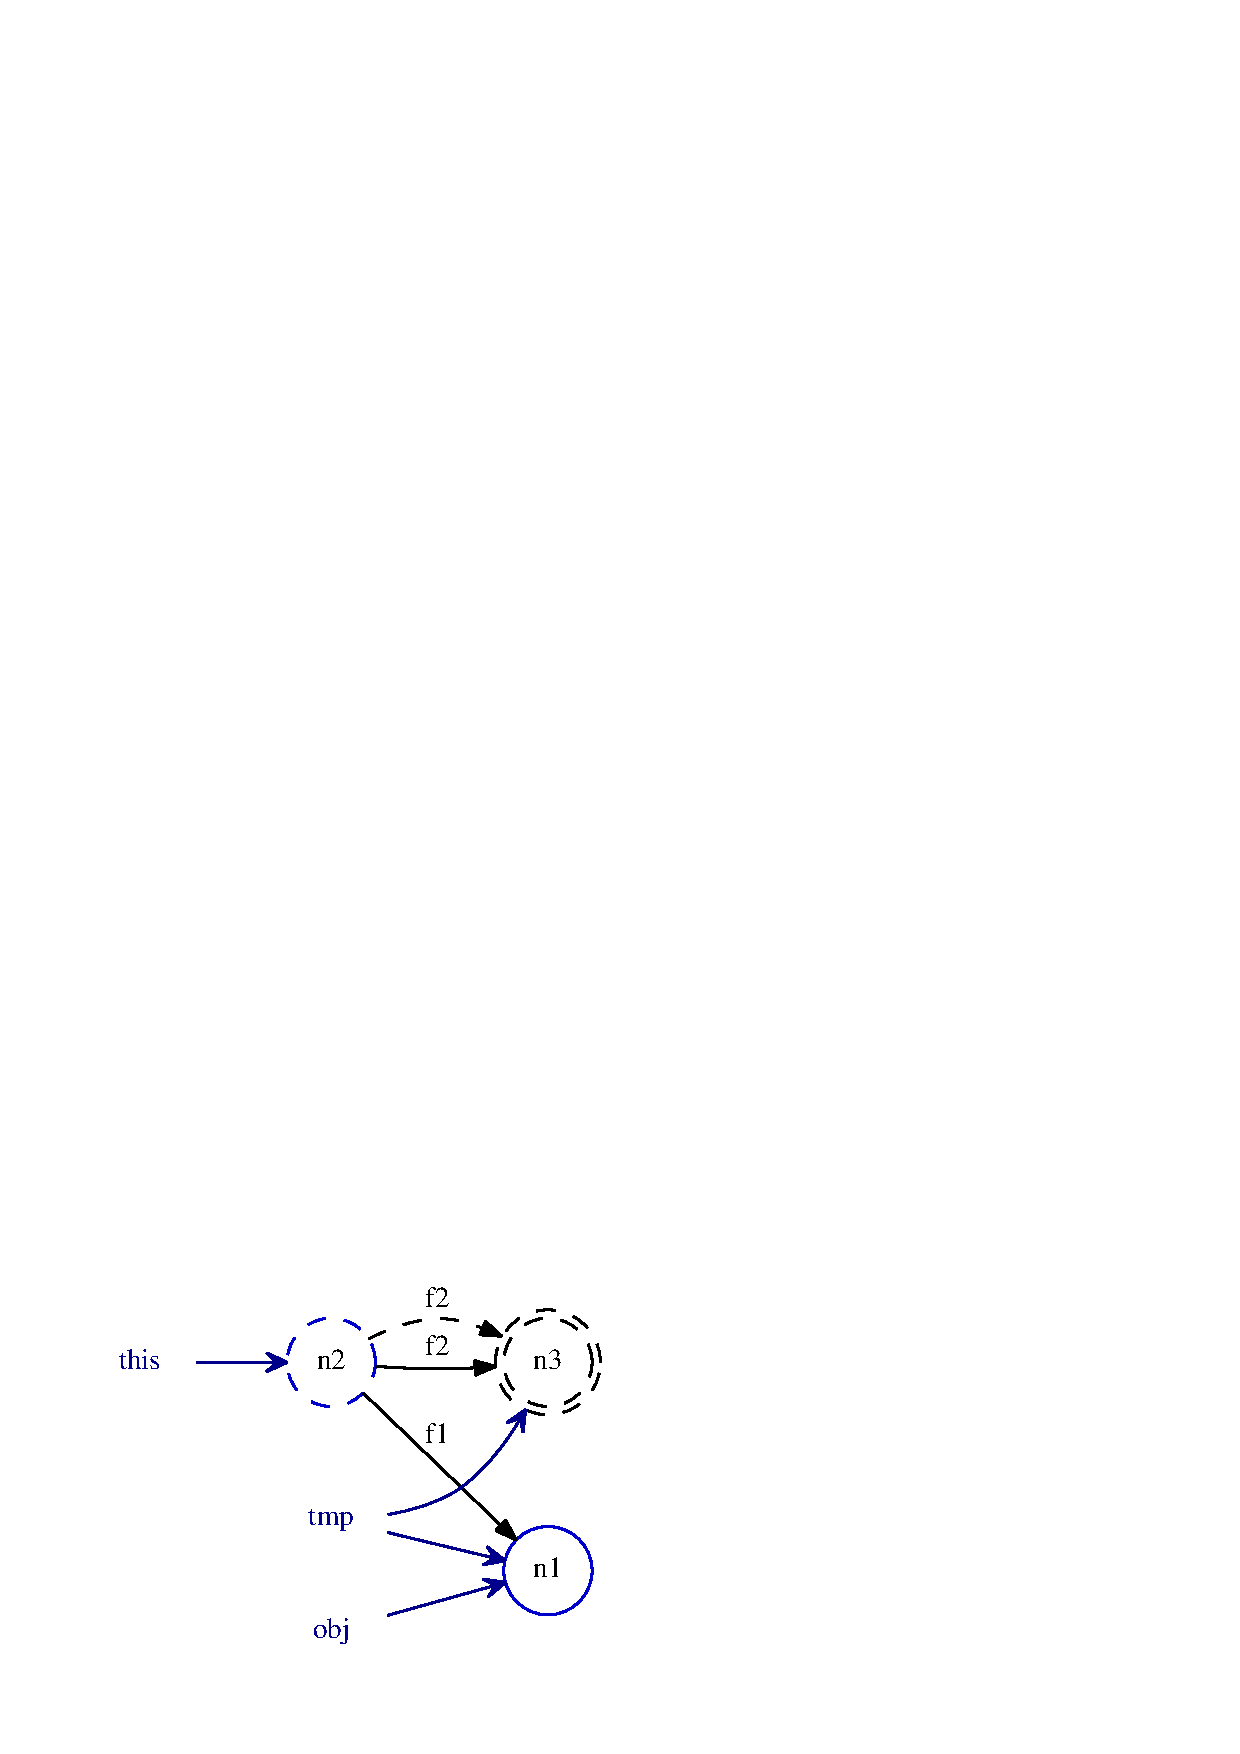
\includegraphics{images/pt_graph1}

    \caption{Simplified Graph Representation}
    \label{fig:pt:graph1}
\end{figure}

\section{Transfer Function}
\section{Inlining Graphs}

\section{Graph-based Type Analysis}
Even though our global type analysis was flow sensitive, it suffered from
critical imprecision with respect to fields and arguments. For this reason, we
implemented a type analysis based on our graphs. The approach we took is to
attach type information to each node. Since nodes represent objects, this is a
sensible thing to do. The additional information we store alongside each node
is similar to what we used in our previous type analysis: $(T_{sub}, T_{exa})$
a pair of two sets of types $T_{sub}$ and $T_{exa}$ where $T_{sub}$ represents
the set of types from which we need to include subtypes, and $T_{exa}$.
The set of runtime types attached to each node is determined based on the node
types. Figure~\ref{fig:pt:types} illustrates the main cases. We then use those
types in order to compute the set of potential targets for a method call. Given
the call \verb/obj.foo()/, we obtain the set of runtime types corresponding to
\verb/obj/ as follows:
$$
    types(\verb/obj/) = \bigcup \{ types(n) ~|~ n \in nodes(\verb/obj/) \}
$$
we can then look for potential targets in the resulting set of types, like we
did in our previous type analysis.


\begin{figure}[h]
    \centering

    \begin{tabular}{ l | l }
        Node Type & Types Associated \\
        \hline
        INode(A)           & $\{\{\}, \{A\}\}$ \\
        LNode(a.f)         & $\{\{type(a.f)\}, \{type(a.f)\}\}$ \\
        PNode(arg)         & $\{\{type(arg)\}, \{type(arg)\}\}$ \\
        OBNode(A)          & $\{\{\},   \{A\}\}$ \\
        NNode              & $\{\{\},   \{\}\}$ \\
        GBNode             & $\{\{Object\},   \{Object\}\}$ (all)\\
        Literal Nodes      & $\{\{\},   \{type(Literal)\}\}$\\
    \end{tabular}

    \caption{Types associated to nodes}
    \label{fig:pt:types}
\end{figure}

If we consider that each field read yield a \emph{load node}, and that every
arguments become \emph{parameter nodes}, this type analysis is exactly as
precise as the one described previously. The main difference comes when those
graphs get inlined. Indeed, during inlining, parameter nodes are mapped to
other nodes at the call site, and load nodes are resolved. The natural inlining
of methods makes this type analysis context sensitive. We consider in
Figure~\ref{fig:pt:precise} an example illustrating this improvement in precision.

\begin{figure}[h]
    \centering
\begin{lstlisting}
class A {
  var f: A = null
  def setF(a: A) { f = a }

  def test(obj: A) {
    val a = new A
    a.setF(a)
    a.f.foo()
  }
  def foo() {
    println("A")
  }
}

class B extends A {
  override def foo() {
    println("B")
  }
}
\end{lstlisting}
    \caption{Improved type analysis}
    \label{fig:pt:precise}
\end{figure}

At the time of the call to \verb/a.f.foo()/ we have from the graph at that
program point that \verb/a.f/ is the \emph{inside node} corresponding to the
object from \verb/new A/. We thus obtain $\{ \{\}, \{A\} \}$ for \verb/a.f/ instead of
$\{ \{A\}, \{A\} \}$, which excludes $B.foo$ from the call.
